\chapter{Derivation of Matched filter}
% The digital version of the analog timing techniques that utilize the ADC as a TDC limits the potential of the ADC because the shape information of the digital signal which is valuable to improve the accuracy of signal detection and estimation is ignored. In this section, the time discrimination algorithms that capture the characteristics of the pulse are introduced, which is called ADC-based algorithms. The ADC-based timing algorithms are generally composed of a detector and an estimator. The function of the detector is to take the signal collected by an ADC and determine the presence or absence of a predefined signal from the raw signal contaminated by noise. If a pulse is detected, an estimator is needed to estimate the values of the parameters of the signal by mathematically modeling the signal. In our case, the detector is to determine if a return pulse with certain characteristics (\ie shape, rise time, and pulse width, \etc) exists in the collected signal, and estimate the arrival time of the pulse if it is present. In this section, we will focus on two detection and estimation algorithms: centroid-based detection and estimation algorithm(centroid-method) and Neyman-Pearson(NP) detector (or Matched filter). The principle of the algorithms will be illustrated first followed by the application of the algorithms to simulated signals and/or signals collected from real experiments. The centroid and NP detector will be introduced in Section xx \todo{xxx} and Section \ref{sec:NP}, respectively.
% %%%%%%%%%%%%%
% %% NP detector
% %%%%
% \section{Neyman-Pearson Detection - Matched Filter}\label{sec:NP}

% The Neyman-Pearson(NP) detector was first introduced by Jerzy Neyman and Egon Pearson in 1933.[neyman1933problem]\citep{neyman1933problem}, and it has been proven to be the optimal detector for radar/ laser signal detection [kay1998fundamentals]\cite{kay1998fundamentals}. \todo{add the review to background section} 
% % and has been widely utilized in many applications like target detection, medicine, nuclear energy, gravitational-wave astronomy, \etc\cite{Hoover2000LocatingResponse,Bousselham2007SamplingTiming,seto2001possibility,gronwall2007influence,gu2002detecting,Jordan2009RangeData,roman2000parametric,Ofek2017OptimalDetection,Vio2018MatchedImplementation}. 
% In general, the NP detector conducts a likelihood ratio test(LRT) to detect a known deterministic signal, \ie the signal has no unknown parameters, while in our case, the arrival time and the amplitude of the return pulse are unknown. In that case, a generalized likelihood ratio test(GLRT) is utilized for detection of signals that have unknown parameters. Moreover, the arrival time of signals can also be determined in the detection process, so our signal detection and estimation problem are combined together, and the problem is defined in the next.
% %% problem definition
% \subsection{Problem definition}
% We state the signal $x[n]$ collected by an ADC is composed of a Gaussian distributed white noise under hypothesis $\hzero$, and under hypothesis $\hone$ the signal is the summation of the noise-free return pulse with unknown amplitude, $As[n]$, and white noise following a  Gaussian distribution. Symbolically,
% \begin{align}\label{eq:mf_hypothesis}
% \mathcal{H}_0:x[n]&=w_0[n]  &n=0, 1,\ldots, N-1\\
% \mathcal{H}_1:x[n]&=As[n-n_0]+w_1[n]  &n=0, 1,\ldots, N-1    
% \end{align}
% where $w_0$ and $w_1$ are the white noise under $\hzero$ and $\hone$ with the variance $W$, and $s$ is the template of the transmit signal normalized to unit amplitude which is also called 'kernel'. The kernel is scaled by the unknown amplitude $A$ and it is assumed to be nonzero over the time interval $[0,M-1]$. The index $n$ represents the timestamp of the $n$-th point of the signal with a size of $N$, and $n_0$ stands for the arrival time of the signal. The time period $[0, N-1]$ should cover the signal for all the possible arrival time, \ie $n_0\in[0, N-M]$. \par
% Note in Equation \eqref{eq:mf_hypothesis}\todo{change eq No.}, the noise on each point of a signal is approximated to be Gaussian distributed, even though the shot noise is created with a Poisson distribution. This approximation is explained in [wall1979practical] \cite{wall1979practical} who states that, despite the number of photons follows Poisson statistics, after sufficient integration for a photon detector of more than 10 photons per integration time interval, the distribution is reduced to Gaussian. In our case, the collected number of photons is far beyond 10 when the laser is on, so the Gaussian approximation is valid. In addition, the white noise $w_0$ and $w_1$ usually have different variances because the shot noise induced by the laser pulse also contributes to the variance of $w_1$. However, the $W_1$ is usually unavailable since the pulse-induced shot noise is amplitude depended which is unknown, and the unknown amplitude also makes it difficult to measure the variance of the pulse-induced shot noise with the appearance of the pulse. Therefore, in this study the $w_0$ and $w_1$ are assumed to be identical, denoted by $w$, and they share the same variance $W$. Also. we can see this approximation does not affect the PFA, and has negligible influence on the PD in next few sections. \par
% Next, we introduce the Neyman-Pearson theorem which allows us to decide the hypothesis of a signal.
% % NP theorem
% \subsubsection{Neyman-Pearson Theorem}
% The Neyman-Pearson theorem (NP theorem) states that, to maximize the probability of detection (PD) $P_D$ of a signal for a given probability of false alarm (PFA) $P_{fa}  =\alpha$, decide $\mathcal{H}_1$ if the generalized likelihood ratio $L_G(x)$ is greater than a threshold $\gamma$; otherwise, decide $\mathcal{H}_0$:
% \begin{equation} \label{eq:Lx}
% L_G(x)=\frac{p(\vec{x};n_0,A,\mathcal{H}_1)}{p(\vec{x};\mathcal{H}_0)}\underset{\mathcal{H}_0}{\overset{\mathcal{H}_1}{\gtrless}}\gamma
% \end{equation}
% The threshold $\gamma$ can be derived from the definition of the PFA
% \begin{equation}\label{eq:pfa}
% P_{fa}=\int_{\{\vec{x}:L_G(x)>\gamma\}} p(x;\mathcal{H}_0)dx=\alpha,
% \end{equation}
% and the PD can be obtained by:
% \begin{equation} \label{eq:pd}
% P_D=\int_{\{\vec{x}:L_G(x)>\gamma\}}p(x;n_0, A, \mathcal{H}_1)d\vec{x}
% \end{equation}
% The probability density distribution (PDF)  of signals with unknown parameters $n_0$ and $A$ under hypothesis $\hzero$ and $\hone$ are denoted by $p(\vec{x};n_0, A,\mathcal{H}_1)$ and $p(\vec{x};\mathcal{H}_0)$, respectively, and the vector $\vec{x} = [x[0],x[1],...,x[N-1]]$. The generalized likelihood ratio indicates the likelihood of a signal being $\hone$ versus being $\hzero$, and Inequation \eqref{eq:Lx} is called the generalized likelihood ratio test. After mathematical reorganization, the GLRT is reduced to (the derivation is provided at the end of this chapter.\todo{ref the last page of this chapter}):
% \begin{eqnarray} \label{eq:Tx}
% T(x) &=&\sum_{n=n_0}^{n_0+M-1}x[n]s[n-n_0] \underset{\mathcal{H}_0}{\overset{\mathcal{H}_1}{\gtrless}}\gamma'\\
% \gamma'&=&\frac{A}{2}\sum_{n=0}^{M-1}s^2[n]+\frac{W\ln\gamma}{A}
% \end{eqnarray}
% and Equation\eqref{eq:pfa} is reformed to
% \begin{equation}\label{eq:pfa2}
% P_{fa}=Pr(T(x)>\gamma';\mathcal{H}_0)
% \end{equation}
% where $T(x)$ is the test statistic which needs to be calculated from experiments. Equation\eqref{eq:Tx} indicates the GLRT calculates the cross-correlation of the signal $x$ with the kernel $s$ for all possible $n_0$, and compares the maximum value with the threshold $\gamma'$. If the threshold is exceeded, a pulse is claimed to be present, and the arrival time $n_0$ is equal to the timestamp of the maximum value. Otherwise, noise is claimed detected. Mathematically, the test statistic can also be written as
% \begin{align}\label{eq:MF_Tx_argmax}
%     T(x)&=\max_{n_0\in[0,N-M]}\sum_{n=n_0}^{n_0+M-1}x[n]s[n-n_0]\\
%     n_0&= \argmax_{n_0\in[0, N-M]}T(x)
% \end{align}
% In practice,  $T(x)$ can be obtained from the convolution of a signal with the conjugated time-reversed kernel $s'[n]$, \ie for each timestamp $n$, the convolution result is
% \begin{align}\label{eq:MF_conv}
% y[n]&=\sum_{m=0}^nx[m]s'[n-m]\\
% s'[n]&=s[N-1-n]
% \end{align}
% and Equation\eqref{eq:MF_conv} is known as the \emph{matched filter} (MF). The matched filter is proved mathematically equivalent to the correlation between the signal and the kernel. For the difference between the correlation approach and the matched filter readers could refer to [Kay, book]\todo{add kay book Vol II}for details.\par
% The time complexity of the MF is a concern for the convolution approach. The time complexity of the MF can be calculated by $\mathcal{O}(MN)$($M$ and $N$ are the numbers of points of the kernel and the signal, respectively). Therefore, the MF could be computationally intensive if a large number of data points are involved in the computation. To accelerate the computation, the MF can be implemented in the frequency domain by using Fast Fourier Transformation (FFT) of which the time complexity is $\mathcal{O}(N\log N)$. However, one should note that if only a few data points are contained in a signal, the FFT approach could be more time-consuming than the brute-force computation. However, one benefit of implementing the MF in the frequency domain is that the arrival time less than the ADC sampling interval can be resolved, which can improve the measurement resolution. 

% % PDF
% \subsubsection{PDF of $T(x)$}
% Now, the original GLRT (Equation \eqref{eq:Lx}) is reduced to a problem that compares the $T(x)$ with a new threshold $\gamma'$ (Equation\eqref{eq:Tx} and Equation \eqref{eq:MF_Tx_argmax}). Now, we need to determine the threshold $\gamma'$ using Equation \eqref{eq:pfa2} for a given $P_{fa} = \alpha$, for which the PDFs of $T(x)$ under both hypothesis $\hzero$ and $\hone$ are required. Since $T(x)$ is a linear combination of Gaussian distributed variables, the PDFs of $T(x)$ should also follow a Gaussian distribution. The estimation of the mean $\hat{\mu}$ and the variance $\hat{\sigma}^2$ for hypothesis $\hzero$ and $\hone$ are shown below, of which the derivation is given at the end of this chapter\todo{refer to last page of the chapter}:
% \begin{align} \label{eq:pdfTx}
% \hat{\mu_0}&=0\\
% \hat{\sigma_0^2}&=W\sum_ns[n]^2\\
% \hat{\mu_1}&=A\sum_ns^2[n]\\
% \hat{\sigma_1^2}&=W\sum_ns^2[n],
% \end{align}
% and the PDFs of $T(x)$ follow:
% \begin{align}
% \mathcal{H}_0: & T(x)\sim N(\hat{\mu_0}, \hat{\sigma}_0^2)\\
% \mathcal{H}_1: & T(x)\sim N(\hat{\mu_1}, \hat{\sigma}_1^2)
% \end{align}
% Or, the normalized test statistic $T'(x) = \frac{T(x)-\hat{\mu}}{\hat{\sigma}^2}$ follows the standard normal distribution $\mathcal{N}(0,1)$.
% % threshold
% \subsubsection{Estimation of threshold $\gamma'$}
% Having the PDF of $T(x)$, Equation \eqref{eq:pfa2} can be expressed by
% \begin{align} \label{eq:pfa_gamma}
% \begin{split}
% P_{fa}&=Pr(T(x)>\gamma';\mathcal{H}_0)\\
% &=Pr(T'(x)>\frac{\gamma'-\hat{\mu}_0}{\hat{\sigma}_0};\mathcal{H}_0)\\
% & = Q(\frac{\gamma'-\hat{\mu}_0}{\hat{\sigma}_0})
% \end{split}
% \end{align}
% where 
% \begin{align}
% \begin{split}
% Q(x) &=\int_x^\infty\frac{1}{\sqrt{2\pi}}\exp(-\frac{1}{2}t^2)dt\\
% &=\frac{1}{2}[1-erf(\frac{x}{\sqrt{2}})]\\
% &=\frac{1}{2}erfc(\frac{x}{\sqrt{2}})\\
% &=1-\Phi(x)
% \end{split}
% \end{align}
% and $\Phi(x)$ is the cumulative distribution function(CDF) for a standard normal distributed variable, and $Q(x)$ is the complementary cumulative distribution function(CCDF). Then, we can derive the expression of $\gamma'$
% \begin{align} \label{eq:MF_gamma'}
% \gamma'=\hat{\sigma}_0Q^{-1}(P_{fa})+\hat{\mu}_0    
% \end{align}
% Here, we can see the PFA is not a function of the amplitude $A$ or the variance of $\hone$signal $w_1$, which means the amplitude of a signal and the variance will not affect the FPA. However, the PD could be affected. The theoretical PD can be obtained from \eqref{eq:pd}
% \begin{align}
% \begin{split} \label{eq:MF_pd}
% P_d&=Pr(T(x)>\gamma';n_0,A, \mathcal{H}_1)\\
% &  = Pr(T'(x)>\frac{\gamma'-\hat{\mu}_1}{\hat{\sigma}_1};n_0,A, \mathcal{H}_1)\\
% & = Q(\frac{\gamma'-\hat{\mu}_1}{\hat{\sigma}_1})\\
% &=\frac{1}{2}erfc(\frac{\gamma-\hat{\mu}_1}{\sqrt{2}\hat{\sigma_1}})
% \end{split}
% \end{align}
% Plugging Equation \eqref{eq:MF_gamma'} in Equation \eqref{eq:MF_pd}, we have
% \begin{align} \label{eq:MF_deflectCoef}
% P_d &= Q(Q^{-1}(P_{fa})-\sqrt{d^2})\\    
% d^2 &= \frac{A^2s^2[n]}{W}
% \end{align}
% where $d^2$ is the deflection coefficient, which can be interpreted as the normalized difference between the PDF of $T(x)$ under hypothesis $\hone$ and hypothesis $\hzero$ by the variance of the noise. The deflection coefficient illustrates that the separation between the two PDFs, as shown in the schematic Figure \ref{fig:dsquare}. In the case of the deflection coefficient is large, the position of the threshold has less impact on the PD, and the detector is approaching a perfect detector($PD = 1$). However, as shown in Equation \eqref{eq:MF_deflectCoef} the deflection coefficient is a function of the amplitude $A$ and variance $W$of a signal, which means the smaller amplitude and larger variance could move the two PDFs closer which causes a decrease of PD.
% \begin{figure}[t!p]
% \centering
% 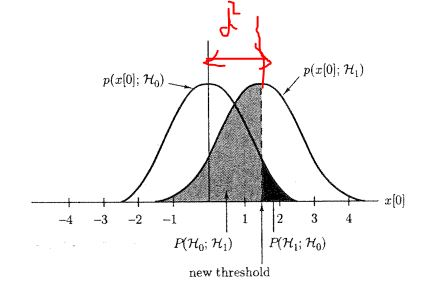
\includegraphics[width=.8\textwidth]{figures/chapter6_ADC/dsquare.jpg}
% \caption{PDF of $\hzero$ and $\hone$, and the deflection coefficient [Ref [Kay book]]}
% \label{fig:dsquare}
% \end{figure}
% % Procedure
% \subsubsection{Procedure of the NP detector}
% Now, we have the problem defined and also the PDFs and the threshold derived. To summarize, the procedure of the NP detector for the signal detection and estimation is following:
% \begin{enumerate}
% \item Find the kernel $s[n]$;
% \item Find the STD of noise $x[n]$;
% \item Calculate the PDFs of the test statistic T(x): Equation \eqref{eq:pdfTx}; \todo{change equation label}
% \item Calculate the threshold $\gamma'$ (threshold for $T(x)$): Equation\eqref{eq:MF_gamma'};
% \item Calculate the $T(x)$ over all possible $n_0$ by convoluting the input signal $x$ and the kernel $s$, and find the maximum value of $T(x)$ and the corresponding $n_0$: Equation\eqref{eq:MF_Tx_argmax} and Equation \eqref{eq:MF_conv};
% \item Compare the maximum value of $T(x)$ with the threshold $\gamma'$, and decide the hypothesis of the signal: Equation \eqref{eq:Tx};
% \item If $\hone$, estimate the arrival time $n_0$: Equation \eqref{eq:MF_Tx_argmax}.
% \end{enumerate}

% \subsection{Application to simulated signals}

% \subsection{Application to real signals}



% derivation
\subsection{Derivation}
\subsubsection{Hypothesis}
\begin{align}\label{eq:mf_hypothesis}
\mathcal{H}_0:x[n]&=w_0[n]  &n=0, 1,\ldots, N-1\\
\mathcal{H}_1:x[n]&=As[n-n_0]+w_1[n]  &n=0, 1,\ldots, N-1    
\end{align}
where $n_0\in[0, N-M]$, $s[n]$ is nonzero over the time interval $[0,M-1]$, and noise $w_0 = w_1\sim\mathcal{N}(0,\sigma^2)$, where the variance $\sigma^2 = W$. The PDF $p(x)$ of a Gaussian distributed variable $x$ is expressed by
\begin{align}
p(x)=\frac{1}{\sqrt{2\pi\sigma^2}}exp[-\frac{1}{2\sigma^2}(x-\mu)^2]
\end{align}
% PDF
\subsubsection{PDF and GLRT}
The PDF for $\hone$ hypothesis: \textcolor{red}{Ref: P67, P253,  P258-260}
\begin{align}
\begin{split}
p(\vec{x};n_0,A,\mathcal{H}_1)&=\prod_{n=0}^{N-1} p(x[n];n_0,A,\mathcal{H}_1)\\
&=\prod_{n=0}^{n_0-1}\frac{1}{\sqrt{2\pi\sigma^2}}exp\big(-\frac{1}{2\sigma^2}x^2[n]\big)\\
&\times \prod_{n=n_0}^{n_0+M-1}\frac{1}{\sqrt{2\pi\sigma^2}}exp\big(-\frac{1}{2\sigma^2}(x[n]-As[n-n_0])^2\big)\\
&\times \prod_{n=n_0+M}^{N-1}\frac{1}{\sqrt{2\pi\sigma^2}}exp\big(-\frac{1}{2\sigma^2}x^2[n]\big)\\
&=\prod_{n=0}^{N-1}\frac{1}{\sqrt{2\pi\sigma^2}}exp\big(-\frac{1}{2\sigma^2}x^2[n]\big)\\
&\times \prod_{n=n_0}^{n_0+M-1}\frac{1}{\sqrt{2\pi\sigma^2}}exp\big(-\frac{1}{2\sigma^2}(-2Ax[n]s[n-n_0]+A^2s^2[n-n_0])\big)
\end{split}
\end{align}
The PDF for $\hzero$ hypothesis:
\begin{align}
\begin{split}
p(\vec{x};\mathcal{H}_0)&=\prod_{n=0}^{N-1} p(x[n];\mathcal{H}_0)\\
&=\prod_{n=0}^{N-1}\frac{1}{\sqrt{2\pi\sigma^2}}exp\big(-\frac{1}{2\sigma^2}x^2[n]\big)
\end{split}
\end{align}
Then, the GLRT can be expressed by:
\begin{align}
\begin{split}
L_G(x)&=\frac{p(\vec{x};n_0,A,\mathcal{H}_1)}{p(\vec{x};\mathcal{H}_0)}\\
&=\prod_{n=n_0}^{n_0+M-1}exp\big(-\frac{1}{2\sigma^2}(-2Ax[n]s[n-n_0]+A^2s^2[n-n_0])\big)
\end{split}
\end{align}
Taking the logarithm on both sides: 
\begin{align}
-\frac{1}{2\sigma^2}\sum_{n=n_0}^{n_0+M-1}-2Ax[n]s[n-n_0]+A^2s^2[n-n_0]>\ln\gamma
\end{align}
Then, we have
\begin{align}\label{eq:MF_Tx_argmax}
T(x)&=\max_{n_0\in[0,N-M]}\sum_{n=n_0}^{n_0+M-1}x[n]s[n-n_0]>\gamma'\\
\gamma'&=\frac{A}{2}\sum_{n=0}^{M-1}s^2[n]+\frac{W\ln\gamma}{A}
\end{align}

% Gaussian distribution
\subsubsection{Gaussian distribution}
\textcolor{red}{Ref: P101-103}
\begin{align} \label{eq:pdfTx}
\begin{split}
&\hat{\mu_0}=E[T(x)]=E\big[\sum_nw[n]s[n]\big]=\sum_nE\big[w[n]\big]s[n]=0\\
&\hat{\sigma^2_0}=Var\big[T(x)\big]=Var\big[\sum_nw[n]s[n]\big]=\sum_nVar\big[w[n]\big]s^2[n]=W\sum_ns^2[n]\\
&\hat{\mu_1}=E[T(x)]=E\big[\sum_n(As[n]+w[n])s[n]\big]=\sum_nE\big[As^2[n]+w[n]s[n]\big]=\sum_nAs^2[n]\\
&\hat{\sigma^2_1}=Var[T(x)]=Var\big[\sum_n(As[n]+w[n])s[n]\big]=\sum_nVar\big[As^2[n]+w[n]s[n]\big]\\
&=0+\sum_nVar\big[w[n]s[n]\big]=W\sum_ns^2[n]
\end{split}
\end{align}
Therefore,
\begin{align} \label{eq:pdfTx}
\hat{\mu_0}&=0\\
\hat{\sigma_0^2}&=W\sum_ns^2[n]\\
\hat{\mu_1}&=A\sum_ns^2[n]\\
\hat{\sigma_1^2}&=W\sum_ns^2[n],
\end{align}
and the PDFs of $T(x)$ follow:
\begin{align}
\mathcal{H}_0: & T(x)\sim N(\hat{\mu_0}, \hat{\sigma}_0^2)\\
\mathcal{H}_1: & T(x)\sim N(\hat{\mu_1}, \hat{\sigma}_1^2)
\end{align}

\subsubsection{Reference for other variables}
\textcolor{red}{PD, PFA and deflection coefficient: P71}